\documentclass[tikz]{standalone}
\usepackage{tikz,tikz-dimline}

% Global settings
\tikzset{
    every picture/.style={
        line width=0.2mm,
        dashed line/.style={dashed, opacity=0.6}
    },
    % Style for centered labels
    area label/.style={
        font=\sffamily,
        align=center
    }
}

% Define semantic color names (keeping exact same RGB values)
\definecolor{senderArea}{RGB}{204,255,204}  % Light green
\definecolor{postageArea}{RGB}{204,229,255} % Light blue
\definecolor{marginArea}{RGB}{255,204,204}  % Light red
\definecolor{codeArea}{RGB}{255,229,204}    % Light orange
\definecolor{readingArea}{RGB}{204,255,255} % Light cyan

\begin{document}
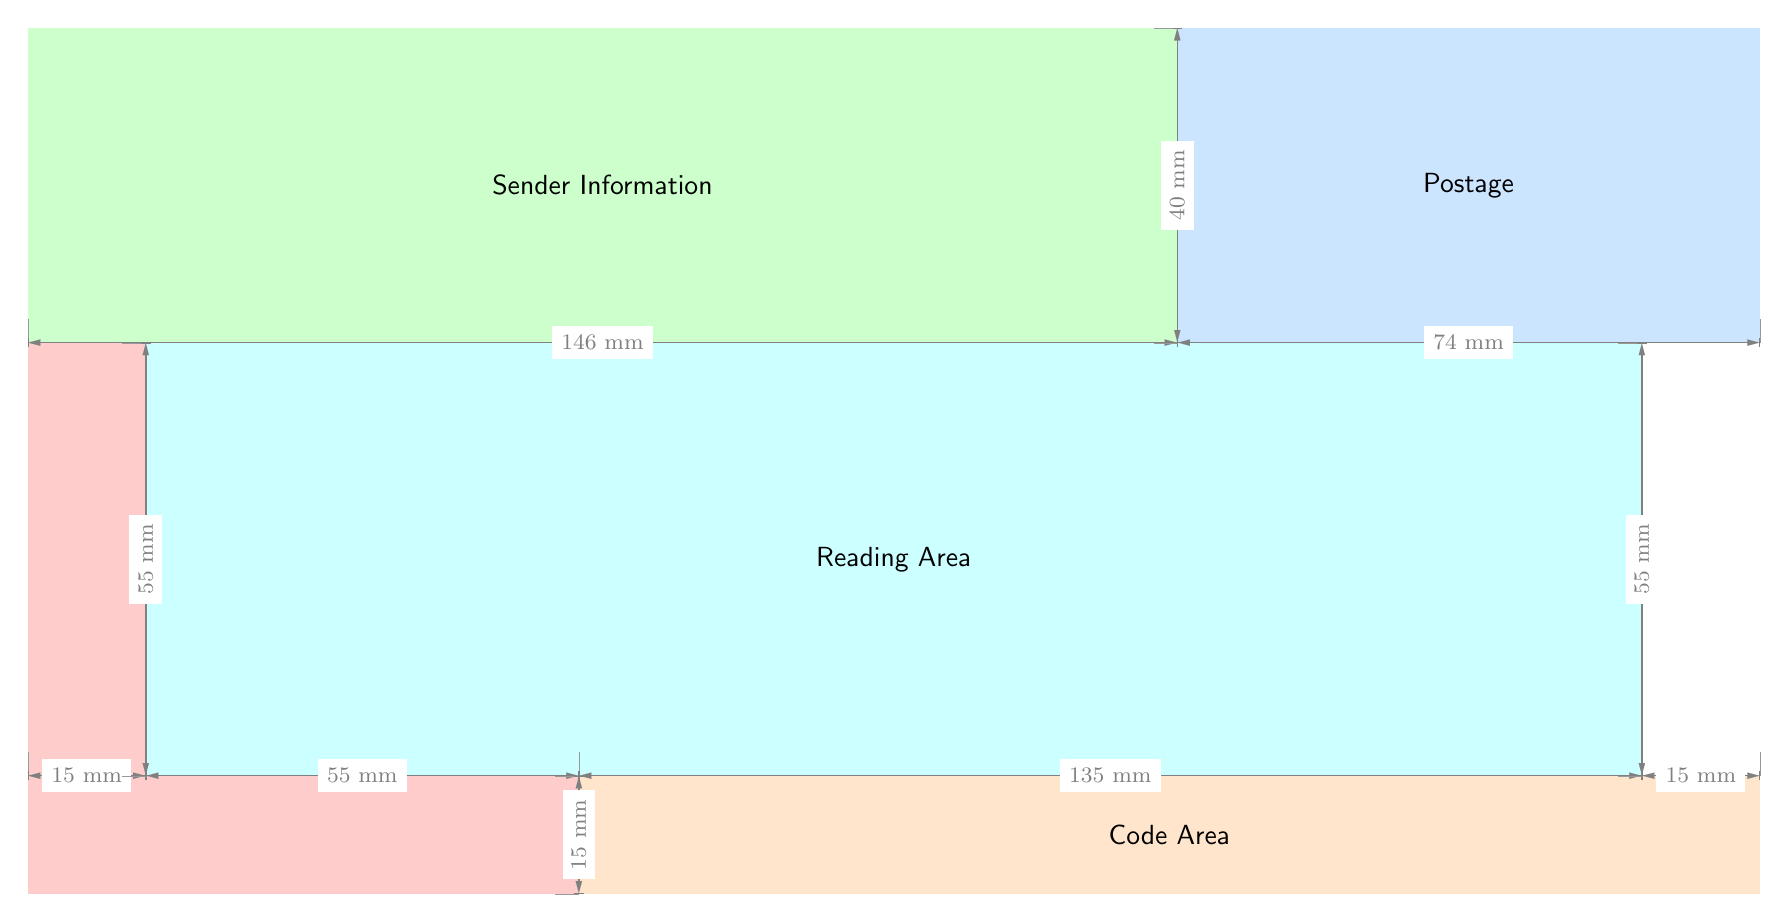
\begin{tikzpicture}[x=1mm,y=1mm]

% Set the canvas size
\path[use as bounding box] (0,0) rectangle (220,110);

% Draw all filled areas with centered labels
\fill[senderArea] (0,70) rectangle ++(146,40);
\node[area label] at (73,90) {Sender Information};


\fill[postageArea] (146,70) rectangle ++(74,40);
\node[area label] at (183,90) {Postage};

\fill[marginArea] (0,0) rectangle ++(15,70);
\fill[marginArea] (15,0) rectangle ++(55,15);

\fill[codeArea] (70,0) rectangle ++(150,15);
\node[area label] at (145,7.5) {Code Area};

\fill[readingArea] (15,15) rectangle ++(190,55);
\node[area label] at (110,42.5) {Reading Area};

%horizontal lines
\dimline[line style = {line width=0.2mm, color=gray},
  extension start length=-0.3cm,
  extension end length=-0.3cm,
  label style={font=\footnotesize}
]{(0,70)}{(146,70)}{146 mm}

\dimline[line style = {line width=0.2mm, color=gray},
  extension start length=-0.3cm,
  extension end length=-0.3cm,
  label style={font=\footnotesize}
]{(146,70)}{(220,70)}{74 mm}

\dimline[line style = {line width=0.2mm, color=gray},
  extension start length=-0.3cm,
  extension end length=-0.3cm,
  label style={font=\footnotesize}
]{(0,15)}{(15,15)}{15 mm}

\dimline[line style = {line width=0.2mm, color=gray},
  extension start length=-0.3cm,
  extension end length=-0.3cm,
  label style={font=\footnotesize}
]{(15,15)}{(70,15)}{55 mm}

\dimline[line style = {line width=0.2mm, color=gray},
  extension start length=-0.3cm,
  extension end length=-0.3cm,
  label style={font=\footnotesize}
]{(70,15)}{(205,15)}{135 mm}

\dimline[line style = {line width=0.2mm, color=gray},
  extension start length=-0.3cm,
  extension end length=-0.3cm,
  label style={font=\footnotesize}
]{(205,15)}{(220,15)}{15 mm}

%vertical linds

\dimline[line style = {line width=0.2mm, color=gray},
  extension start length=-0.3cm,
  extension end length=-0.3cm,
  label style={font=\footnotesize}
]{(146,70)}{(146,110)}{40 mm}

\dimline[line style = {line width=0.2mm, color=gray},
  extension start length=-0.3cm,
  extension end length=-0.3cm,
  label style={font=\footnotesize}
]{(15,15)}{(15,70)}{55 mm}

\dimline[line style = {line width=0.2mm, color=gray},
  extension start length=-0.3cm,
  extension end length=-0.3cm,
  label style={font=\footnotesize}
]{(205,15)}{(205,70)}{55 mm}

\dimline[line style = {line width=0.2mm, color=gray},
  extension start length=-0.3cm,
  extension end length=-0.3cm,
  label style={font=\footnotesize}
]{(70,0)}{(70,15)}{15 mm}

\end{tikzpicture}
\end{document}